\chapter{Revisão de Literatura}\label{cap:revisaolit}
Este capítulo apresenta uma revisão dos principais conceitos relacionados ao tema deste trabalho, envolvendo Arquitetura Orientada a Serviço, Tecnologia Web Service e da Segurança Aplicada a SOA.

\section{Arquitetura orientada a serviços}

%A Arquitetura Orientada a Serviços (SOA) estabelece um modelo arquitetônico que visa aprimorar a eficiência, agilidade e a produtividade de uma empresa, posicionando os serviços como os principais meios para que a solução lógica seja representada no suporte à realização dos objetivos estratégicos associados à computação orientada a serviços \cite{ERL09}.

A Arquitetura Orientada a Serviços (SOA) , consiste em uma coleção de componentes distribuídos que fornecem e ou consomem serviços~\cite{Clements2010}, tem sido amplamente utilizada por um grande número de empresas.

Serviços correspondem a recursos de software bem definidos através de uma linguagem padrão, são auto-contidos,  proveem funcionalidades padrões do negócio, independentes do estado ou contexto de outros serviços~\cite{Furtado2009}.

SOA pode ser caracterizada como uma arquitetura corporativa onde serviços podem ser criados, reutilizados e facilmente compartilhados entre aplicações. Neste caso as funcionalidades de um sistema são decompostas em serviços interoperáveis o que permite a integração entre aplicações. O objetivo da SOA é estruturar sistemas distribuídos com base nas abstrações de regras e funções de negócio~\cite{Josuttis07}.

Existem muitas definições para SOA, no entanto elas possuem pontos em comuns pois em todos os conceitos são abordados temas que remetem ao compartilhamento do serviços, da independência da plataforma e linguagem de programação, da possibilidade de flexibilidade e agilidade no desenvolvimento de uma aplicação para gerenciar um negócio~\cite{ERL09}.
Segundo~\cite{Josuttis07}, o funcionamento de SOA baseia-se em três conceitos: serviços, interoperabilidade e baixo acoplamento.

Por serviços entende-se SOA como uma arquitetura neutra, que objetiva abstrair a realidade, concentra-se nos aspectos do negócio, possibilitando que sistemas sejam construídos em plataformas diferentes, tendo como finalidade a redução de problemas de integração, uma vez que isso  pode ser feito de forma flexível por meio dos serviços disponibilizados na arquitetura. Portanto, serviço pode ser visto como um conjunto de funções, abstrações de funcionalidades de negócios de um sistema com uma interface bem definida.

A interoperabilidade visa à integração entre esses sistemas e representa um objetivo fundamental da orientação a serviços, pois estabelece uma base para a realização de outros objetivos e benefícios estratégicos. Isso é possível, pois uma das características de SOA é que seus serviços são reutilizáveis, possuem baixo acoplamento, tem contratos formais e são independentes. Logo, uma vez que esses serviços estejam disponíveis aos clientes eles não precisam conhecer a lógica ou os processos de negócio para consumir e integrar serviços a suas aplicações.

O baixo acoplamento ou acoplamento fraco é um conceito vital para o funcionamento de um sistema distribuído, uma vez que ele determina que diferentes partes e funcionalidades de um sistema sejam independentes umas das outras, dessa maneira, alterações ou problemas em uma determinada parte do sistema não trará consequências para o resto do sistema, trazendo benefícios como escalabilidade, flexibilidade e tolerância a falhas. Acoplamento fraco refere-se a uma abordagem em que as interfaces podem ser desenvolvidas com o mínimo de suposições mútuas entre o emissor e os destinatários, reduzindo assim o risco de que uma mudança em um aplicativo ou módulo force uma mudança em outra aplicação ou módulo.

Segundo~\cite{Bianco2007}, SOA é um estilo arquitetural e para implementá-lo podem ser usadas diversas tecnologias tais como RMI ( \emph{Remote Method Invocation}), CORBA (\emph{Common Object Request Broker Architecture}), DCOM (\emph{Distributed Component Object Model}), REST (\emph{Representational State Transfer}) e  Web Services, que é uma das principais tecnologias para implementação desses serviços.

A abordagem de arquiteturas orientadas a serviços (SOA) e de Web Services estão centradas no conceito de serviço, tanto no nível de negócios quanto no nível tecnológico, e compartilham os mesmos princípios.

Apesar de SOA e Web Service compartilharem os mesmos princípios, SOA representa propositadamente uma tecnologia neutra, a definição de Web Service destaca o papel central das tecnologias da Web específicas.

%, a saber: o Identificador Uniforme de Recursos, e os protocolos de Internet, que oferecem, respectivamente, a identificação uniforme, mecanismos de comunicação e o XML, que é usado para definir e descrever a interface do aplicativo, bem como para codificar as mensagens trocadas entre o Web Service e seus clientes.

\section{WEB SERVICES}

%A seguir será realizada uma abordagem da tecnologia de Web Services, ela será descrita, pois se optou por utilizá-la como modelo a ser implementado como objeto desse trabalho. Outro motivo que originou essa escolha foi a que a Divisão de Tecnologia da Polícia Civil do Distrito Federal apesar de ainda não utilizar SOA adota de forma reduzida a tecnologia de Web Services para integrar seus sistemas legados o que pode facilitar a adequação a futuras mudanças.
%Esta seção descreve os conceitos da tecnologia de web Services, uma vez que se optou por utilizá-la como modelo a ser implementado como objeto desse trabalho. A escolha desta tecnologia foi reforçada devido ao fato da Divisão de Tecnologia da Polícia Civil do Distrito Federal, apesar de ainda não utilizar SOA, adotar de forma reduzida a tecnologia de Web Services para integrar seus sistemas legados o que pode facilitar a adequação a futuras mudanças.

%Web Service (WS) é um sistema de software identificado por um URL, cujas interfaces e ligações com o público são definidos e descritos usando XML. Sua definição pode ser descoberta por outros sistemas de software. Estes sistemas podem então interagir com o WS de uma maneira prescrita por sua definição, usando mensagens baseadas em XML transmitidas por protocolos de Internet.

Web Service pode ser definido como um sistema de software projetado para suportar interações interoperáveis máquina-a-máquina sobre uma rede \cite{Booth2004}.

Um dos fatores da aceitação de Web Services está no fato dele usar protocolos abertos de comunicação na Internet e XML para transacionar o seu negócio.  Um WS é, portanto, um sistema de software que pode agir a pedido de qualquer computador conectado à rede e que se comunica usando padrões XML \cite{Pulier2005}.

Por meio desta tecnologia é possível promover a interoperabilidade entre aplicações e que tenham sido desenvolvidos em plataformas diferentes tornando-as compatíveis permitindo que as aplicações enviem e recebam dados em formatos variados. Cada aplicação pode ter a sua própria linguagem, que é traduzida para uma linguagem universal, como é o caso do formato XML.

A abordagem de arquiteturas orientadas a serviço e Web Services estão centradas no conceito de serviço, tanto a nível de negócios  quanto a nível tecnológico, e compartilham os mesmos princípios~\cite{Bertino2010}. Dentre os princípios que mais se destacam podem ser citados:

\begin{itemize}
    \item Autonomia de serviço: Para os serviços realizarem suas capacidades de modo consistente e confiante, sua lógica precisa ter um grau significativo de controle sobre seu ambiente e recursos~\cite{ERL09}.

    \item Baixo acoplamento: Acoplamento refere-se a uma conexão do relacionamento entre dois elementos. Uma medida de acoplamento se compara a um nível de dependência~\cite{ERL09}. De outra forma pode dizer que o baixo acoplamento refere-se a uma abordagem em que as interfaces podem ser desenvolvidas com a mínima dependência uma das outras o que reduz o risco  de uma mudança e qualquer uma das partes forçar a mudança na outra parte não modificada.

    \item Contrato formal: O contrato informa o que o Serviço faz e como ele se comunica (o que deve receber e o que deve entregar). Em outras palavras Contratos são documentos textuais que descrevem o que o serviço faz e eles são o foco do design de serviço, porque regem praticamente tudo que é feito pelos serviços~\cite{ERL09}. Logo, todo serviço possui um contrato entre o requisitante e o provedor deste serviço.

\end{itemize}

Segundo~\cite{Bertino2010}, cada organização tem que ter autonomia para exercer um controle independente sobre os seus serviços. Para isso a autonomia do negócio tem que ser correspondente a do Web Service no momento do oferecimento e execução do serviço.
%\begin{itemize}
    %\item Um Web Service deve possuir seus próprios dados, não deve compartilhar suas informações internas com outros Web Services, nem ter um armazenamento de dados comum;

    %\item As comunicações entre os serviços devem ser explícitas e de acordo com seu contrato publicado (interface). Autonomia de um serviço no nível do negócio requer um acoplamento flexível a nível técnico. Desta forma, as dependências entre os consumidores e os serviços estão limitadas a conformidade dos consumidores para o contrato de serviço.

%\end{itemize}

%A plataforma de Web Services é definida por vários padrões da indústria suportados por todas as comunidades de fornecedores. Essa plataforma está associada à coleção de padrões e especificações de tecnologias abertas tais como XML - Shema Definition Language, SOAP - Simple Object Access Protocol, Description Langue(WSDL)e  UDDI (Universal Description, Discovery). Nas seções a seguir será feito uma descrição de cada uma dessas tecnologias.
A plataforma de Web Services é definida por vários padrões da indústria suportados por todas as comunidades de fornecedores. Essa plataforma está associada à coleção de padrões e especificações de tecnologias abertas tais como Simple Object Access Protocol (SOAP), Web Services Description Language (WSDL) e  Universal Description and Discovery Information (UDDI). Nas seções a seguir será feito uma descrição de cada uma dessas tecnologias.

%\subsection{Extensible Markup Language-XML}

%XML(eXtensible Markup Language), é uma linguagem de marcação recomendada pela W3C para a criação de documentos sendo amplamente utilizada em Web services. Ele é composto por tags que podem ser determinados livremente pelo usuário em seu documento XML, o que não ocorre na HTML (HyperText Markup Language)  que também possui tags predefinidas. A linguagem XML pode ser classificada como extensível, pois permite definir os elementos de marcação além de ser utilizado para definir a forma como os dados trocados entre aplicações devem ser estruturados, isso é possível por meio de um formato único de apresentação que permite descrever os dados e também a forma que eles serão apresentados.

%A linguagem HTML possui limitações e o XML foi concebido com intuito de resolver esse problema, sendo desenvolvido para melhorar o suporte à criação e o gerenciamento de conteúdos dinâmicos. Ele é uma linguagem baseada em texto e totalmente independente da plataforma, sendo ideal para troca de mensagens entre plataformas que podem ser distintas ou não. Além disso, ele possui uma gramática rigorosa o que permite construir analisadores XML que podem ler qualquer documento XML.

%O XML pode ser utilizado em uma grande variedade de transações e publicações de dados, haja vista que ele possui uma forma simples de escrever dados atribuindo significados \cite{Hunter2007}. Ele tem vantagens distintas quando comparado a outras formas de representação de dados tais como:

       % \begin{itemize}
       %     \item XML pode ser entendido tanto por pessoas quanto por máquinas haja vista que sua leitura é de fácil compreenção;

       %    \item O número de plataformas que suportam XML e são capazes de realizar atividades de leitura, escrita e manipulação de dados nesse formato são relativamente grandes;

       %    \item As comunicações entre os serviços devem ser explícitas e de acordo com seu contrato publicado (interface). Autonomia de um serviço no nível do negócio requer um acoplamento flexível a nível técnico. Desta forma, as dependências entre os consumidores e os serviços estão limitados a conformidade dos consumidores para o contrato de serviço.
       % \end{itemize}

%Porém, há algumas desvantagens na utilização dessa linguagem de marcação, a primeira refere-se ao tamanho dos arquivos que são grandes devido a sua natureza descritiva, uma outra está associada ao consumo elevado de processamento para a sua interpretação. Visando reduzir estes problemas, vários mecanismos têm sido desenvolvidos. Um exemplo são interpretadores de XML aprimorados.

\subsection{Simple Object Accesss Protocol (SOAP)}
SOAP é um protocolo de transporte que é responsável pela troca de mensagens entre aplicações em ambientes distribuídos e descentralizados, ele segue um padrão que foi especificado pelas normas da W3C, sendo baseado em XML o que o torna totalmente compatível com qualquer plataforma e com linguagens que tenham suporte para a manipulação de arquivos XML. Seu conteúdo é composto por informações e estruturas de dados~\cite{COYLE}.

A estrutura de uma mensagem SOAP é definida em um documento XML, sua estrutura possui os seguintes elementos:\emph{ envelope, body} que são obrigatórios e \emph{header e fault} que são opcionais. As seguir uma breve descrição desses elementos:

 \begin{itemize}
            \item \emph{Envelope}: Este é o elemento raiz da mensagem SOAP sendo responsável por identificar o documento XML com uma mensagem SOAP e por definir o conteúdo da mensagem;

            \item \emph{Header} (opcional): Contêm os dados do cabeçalho, este elemento possui informações especificas do aplicativo da mensagem SOAP;

            \item \emph{Body}: Contém as informações de chamada e resposta ao servidor, ele contém a mensagem SOAP pretendida que o usuário espera;

            \item \emph{Fault}: Este elemento possui as informações dos erros ocorridos no envio da mensagem. Esse elemento só aparece nas mensagens de resposta do servidor.

 \end{itemize}


\subsection{Web Services Description Language (WSDL)}

Web Services Description Language (WSDL) é uma linguagem para descrição de serviços escrita em XML. Nela são descritos os serviços externos, ou interfaces que são oferecidos por uma determinada aplicação, independente de sua plataforma ou linguagem de programação. Além disso, ela contém as especificações de localização das operações (métodos ou serviços) que fazem parte dos Web Services. Atualmente, ela encontra-se na versão 2.0.

WSDL podem ser mapeados para qualquer linguagem de implementação, plataforma, modelo de objeto e ou sistema de mensagens \cite{Bertino2010}. Ele é caracterizado por uma parte abstrata, onde é descrita a interface do serviço e outra concreta local onde são definidos os protocolos de conexão e outras informações, conforme Figura~\ref{fig:composicao_WSDL}.

A parte abstrata é constituída pelos seguintes elementos: Tipos, que são elementos que definem os tipos de dados usados pelos Web Services, neles são especificados os tipos que serão trocados nas mensagens de entrada e saída do serviço; Mensagem, que é um elemento que permite descrever de forma abstrata os dados que serão transmitidos entre o serviço e o consumidor do serviço; Operações, que é um elemento que é semelhante à definição de um método, no entanto, ele só permite que você defina a entrada, saída e mensagens de erro que estão associados com uma operação e PortType, que são conjuntos de operações abstratas, que são suportadas por um serviço, cada um contendo mensagens de entrada e saída.

A parte concreta do WSDL, local de definição do protocolo e do endereço onde o serviço estará disponibilizado, compõe-se pelos seguintes elementos: O binding (ligação), que é o elemento que é responsável por ligar os elementos abstratos e concretos em um documento WSDL e de fornecer detalhes de como as mensagens serão transmitidas. E os Serviços e Portas, que são elementos que especificam a localização (endereço URL ou e-mail), neste caso, o elemento de serviço atribui um nome para o serviço e o associa a uma interface abstrata e descrevendo o local onde o serviço será acessado.



%\begin{itemize}
%    \item Tipos: São os tipos de dados usados pelo Web Services neles são especificados os tipos que serão trocados nas mensagens de entrada e saída do serviço;

 %   \item Mensagem:  É um elemento  que permite descrever de forma abstrata os dados que serão transmitidos entre o serviço e o consumidor do serviço;

  %  \item Operações:  Este elemento é semelhante a definição de um método, no entanto, ele só permite que você defina a entrada, saída e mensagens de erro que estão associados com uma operação;

   % \item PortType: São conjuntos de operações abstratas, que são suportadas por um serviço, cada um contendo mensagens de entrada e saída.

%\end{itemize}

%No que se refere à parte concreta do WSDL, local no qual são realizados os detalhes de implementação, ela compõem-se pelos seguintes elementos:

%\begin{itemize}
    %\item Ligação (binding): Este elemento liga os elementos abstratos e concretos  em um documento WSDL. O elemento está associada (binding)  a um elemento de (portType) específico, e que também apresenta o endereço do serviço Web que está associado com o elemento (portType). Finalmente, o elemento (binding) mostra o protocolo que é usado para comunicar com o Web Service;

   % \item Service e ports: Estes elementos especificam a localização (endereço URL ou email),neste caso, o elemento de serviço atribui um nome para o serviço e o  associa a uma interface abstrata e descrevendo o local onde o serviço será acessado.

%\end{itemize}

\begin{figure}[!htb]
\centering
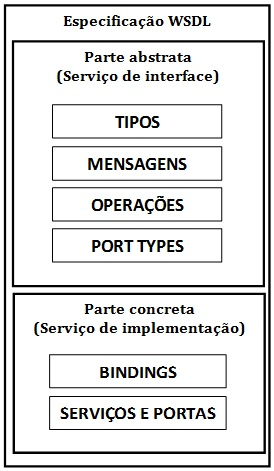
\includegraphics[scale=0.5]{COMPOSICAO_WSDL.jpg}
\caption{Especificação de serviços WSDL, adaptado de~\cite{Bertino2010}}
\label{fig:composicao_WSDL}
\end{figure}


\subsection{Universal Description, Discovery and Integration (UDDI)}

UDDI é um componente importante da arquitetura de Web Services, sendo formado por um serviço de diretório que armazena descrições de serviço. Esse serviço obedece ao padrão integração, descoberta e descrição universal. Além disso,  ele prescreve o layout de um banco de dados que contém  descrições de serviços que permitirão a clientes de serviços web procurar serviços relevantes~\cite{TANENBAUM2007}.

O UDDI provê um método padronizado para a publicação e descoberta de informações, permitindo que as empresas tanto publiquem como encontrem Web Services. Segundo~\cite{Cerami2002}, os dados capturados dentro de UDDI são divididos em três categorias principais:

\begin{enumerate}[a )]
	\item Páginas brancas: Esta categoria inclui informações gerais tais como nome, descrição e endereço dentre outras informações sobre o fornecedor do serviço;

	\item Páginas amarelas: Esta categoria inclui dados de classificação geral para qualquer empresa ou serviço oferecido. Por exemplo, esses dados podem incluir a indústria, o produto, ou códigos geográficos baseados sobre taxionomias padronizadas;

	\item Páginas verdes: Esta categoria inclui informações técnicas sobre um Web Service. Geralmente, essa informação inclui um apontador (ponteiro) para uma especificação externa e um endereço para invocar o serviço.

\end{enumerate}

\section{Representational State Transfer}
A arquitetura \emph{Representational State Transfer (REST)}, foi proposta por Roy Fielding em
2000 em sua tese de doutorado e pode ser descrita como um conjunto de princípios arquiteturais que podem ser utilizados para o desenvolvimento de serviços web e que utilizam o protocolo HTTP para realizar as trocas de mensagens ~\cite{ Fielding2000}.

Dessa forma, para que os princípios arquiteturais que permeiam \emph{REST} sejam seguidos, um conjunto de restrições deve ser implementado ~\cite{ Fielding2000}. Um aplicação que esteja em conformidade com essas restrições, a seguir descritas, são classificadas com RESTfull.~\cite{Richardson2007}

\textbf{Cliente-Servidor:} Essa restrição está associada a separação de interesses, que é o princípio por trás das restrições da arquitetura cliente-servidor. Nela procura-se separar as preocupações relacionadas à interface do usuário das preocupações de armazenamento de dados. Isso permite que os componentes possam evoluir de forma independente melhorando a portabilidade e a escalabilidade das aplicações.

\textbf{\emph{Stateless}:} Diz respeito à interação entre cliente e servidor. Nesse caso, a  comunicação deve ser realizada sem que haja o armazenamento de qualquer tipo de estado no servidor. Sendo assim,  toda informação de estado deve ser conhecida somente pelo cliente.  Esta característica permite a escalabilidade do servidor, uma vez que pode liberar recursos no final de cada pedido.
Contudo, uma desvantagem associado a essa característica  está relacionada à performance da rede, pois em decorrência das constantes requisições com dados repetidos  ela é reduzida.

\textbf{\emph{Cache}:} A utilização do cachê, tem  a finalidade de diminuir o impacto da desvantagem ocasionada pela redução de performance. Uma vez que exige que os dados de uma resposta vinda de uma requisição ao servidor, sejam marcados como \emph{cacheable} (sujeito à utilização do cachê) ou \emph{noncacheable} (não sujeito à utilização do \emph{cache}). Se uma resposta for marcada como cacheable, então ela será reutilizada como resposta em futuras requisições equivalentes, permitindo que o servidor fique mais livre, e portanto, mais escalável, haja vista que algumas interações poderão ser eliminadas por completo o que melhora a eficiência e  performance  de acesso a recursos percebido pelo usuário.

\textbf{Sistema em camadas:} Essa restrição caracteriza-se pela divisão do sistema em camadas hierárquicas, restringindo a visualização dos componentes participantes de forma que cada componente só possa ver a camada com a qual esteja interagindo diretamente. Ao restringir a visibilidade de um sistema a uma única camada, torna-se possível delimitar a complexidade do sistema e promover a independência de cada uma das camadas.  Essa separação permite que  o sistema seja mais robusto e resistente a erros.

\textbf{Code-On-Demand:} Dentre o conjunto restrições propostas pelo estilo REST, esta é aquela que permite a opção de baixar e executar diretamente códigos no  lado cliente, sendo opcional. Com isso, busca-se  obter extensibilidade e simplificar  o cliente. No entanto, isso também reduz a visibilidade.

\textbf{Interface Uniforme:} A principal característica que diferencia o estilo arquitetural REST de outros utilizados em rede é a ênfase  quanto ao uso de uma interface uniforme entre os componentes. Aplicando o princípio de generalização de engenharia de software à interface dos componentes, a arquitetura é simplificada e a visibilidade da interações é melhorada. Contudo, esta generalização pode diminuir a eficiência do sistema, devido à aplicação não poder transmitir a informação num formato especifico de acordo com a sua  necessidade.  Com o objetivo de obter uma interface uniforme, REST define quatro requisitos de interface:

 \begin{itemize}
    \item \textbf{Identificação dos recursos:} Na arquitetura REST, cada recurso deve possuir um  identificador universal  denominado Uniform Resource Identi?er (URI). Que é definido como  uma sequência de caracteres que identi?cam um recurso físico ou abstrato [RFC 3986]. E são utilizados para descoberta de recursos e serviços.
    \item	\textbf{Representação de recursos:} Os recursos devem ser manipulados a partir de suas representações, uma vez que elas podem estar representadas em formatos diferentes formatos, tais como: JSON, XML,PDF, texto puro, etc. É importante frisar que uma aplicação REST não transmite o recurso efetivamente, mas sim a sua uma representação, em um formato pré-acordado entre o cliente e o servidor;
    \item	\textbf{Mensagem auto descritivas:} Os recursos são dissociados da sua representação, haja vista que o seu conteúdo  pode que ser acessado em em formatos diferentes. Dessa forma, as mensagens devem conter metadados que indicam como o conteúdo transmitido deve ser tratado.  Os metadados são utilizados para controlar cache, detectar erros de envio, negociar formatos de uma representação adequada, realizar controle de autenticação e acesso, etc;
    \item	\textbf{Utilização de hipermídia para estado da aplicação:} Neste caso, as representações de recursos obtidas em uma aplicação REST devem possuir \emph{hiperlinks} que permitam a navegação do cliente pelos recursos. Uma vez que o servidor não pode  armazenamento de qualquer tipo de estado. Dessa forma, o Cliente pode interagir com outros recursos existentes sem a necessidade de que ele conheça a relação completa destes recursos pois poderá seguir estas ligações para se deslocar de um recurso para outro.


    %Este pré-requisito é o menos cumprido por aplicações autointituladas RESTful: As representações de recursos obtidas em uma aplicação REST devem possuir hiperlinks que permitam a navegação do cliente pelos recursos. Ou seja, diferentemente de arquiteturas baseadas em RPC (Remote Procedure Call), o cliente não deve conhecer previamente as URIs para os recursos da aplicação (apenas a raiz do serviço), sendo que o servidor deve prover links que permita a descoberta dos recursos pelo cliente; não há contrato do serviço e não há garantia que um recurso em uma determinada URI possa estar disponível no futuro;
\end{itemize}

O protocolo HTTP é o padrão utilizado na arquitetura REST para promover a comunicação entre o cliente e o servidor. Isso se dá pela manipulação dos recursos utilizando os métodos HTTP: GET, POST, PUT ou DELETE.



\section{Segurança em SOA}

\subsection{Conceitos básicos}

Segurança da informação pode ser definida como um conjunto de ações que são executadas com a finalidade de prover segurança às informações de indivíduos e organizações. Atualmente a segurança é um requisito importante para qualquer aplicação distribuída, tais como aplicações governamentais, aplicações de segurança pública e de defesa dentre outros~\cite{Bertino2010}.

A Segurança aplicada a SOA requer o estabelecimento de propriedades básicas, uma vez que os aspectos funcionais aplicados a esta arquitetura são iguais aos de aplicações tradicionais.  Logo, segundo~\cite{Verissimo2001}, a segurança está fundamentada nos seguintes atributos básicos: autenticidade, integridade, confidencialidade e disponibilidade.

No que se refere à autenticidade, este é um atributo que visa estabelecer a origem da informação, buscando verificar a identidade de um usuário. Assim, objetiva-se garantir que o usuário ou serviço é realmente quem diz ser e que tem os privilégios necessários para acessar e ou enviar uma determinada informação.

A integridade é aquela que se preocupa em evitar ou em detectar a modificação não autorizada de informações ou mensagens. Esse atributo busca proteger a mensagem de modificações não permitidas.

A confidencialidade preocupa-se com a proteção contra acessos não autorizados de dados e informações. Segundo~\cite{Bertino2010}, esse atributo procura proteger o conteúdo de uma mensagem ou informação  para que ele não possa ser visualizado no momento da transmissão, exceto por serviços autorizados a visualizá-los por terem a necessidade de ver o conteúdo da mensagem, a fim de realizar o seu encaminhamento.

Finalmente, a disponibilidade está preocupada com a garantia de que os serviços de informação permaneçam acessíveis somente a usuários autorizados. De forma que uma mensagem ou informação uma vez solicitada possa ser prontamente entregue ao destinatário, garantindo assim que os usuários legítimos recebam os serviços a que têm direito. E outra palavras esse atributo busca garantir que a informação estará disponível quando solicitada.

Apesar de compartilhar estes conceitos,  a segurança em SOA exige uma abordagem  diferenciada e outros aspectos devem ser verificados. Um exemplo disto é a proposta de segurança em nível de mensagem.

Segundo~\cite{SOASecurity2008}, a segurança em nível de mensagem busca sanar problemas e complementar a segurança que é oferecida na camada de transporte, que é realizada por meio dos protocolos SSL (\emph{Security Socker Layer}) e TLS (\emph{Transport Layer Security}). Neste caso, os dados são cifrados na camada de transporte sendo estabelecido um canal seguro de comunicação entre dois serviços. Dessa forma, a comunicação ponto a ponto é garantida e segura. Porém, uma vez existindo interfaces intermediárias entre provedor do serviço e o consumidor, o processo de cifrar e decifrar os dados, que ocorre na camada de transporte, irá ocorrer toda vez que os dados trafegarem por um serviço intermediário, isso faz com que o sigilo dos dados e a segurança sejam quebrados em cada serviço intermediário. Para resolver este problema, propõem-se a segurança em nível de mensagem que consiste em utilizar mecanismos de segurança como cifrar partes da mensagem, o que resolve este problema, pois a segurança é fim a fim o que significa dizer que os dados estarão seguros mesmo quando a transmissão envolver um ou mais intermediários.

\subsection{Criptografia}

A palavra criptografia origina do Grego kryptós, ``escondido'', e gráphein, ``escrever'',  e pode ser  conceituada como sendo a ciência a arte de manter mensagens seguras~\cite{Schneier1995}. Ela está  associada a vários aspectos da segurança da informação, tais como: privacidade ou confidencialidade, integridade do dados, autenticação e não-repúdio~\cite{Menezes1996}. Em síntese, o processo de criptografia consiste em transformar uma informação que está em texto claro (\emph{plaintext}), em uma informação cifrada (\emph{ciphertext}), criptografada. O processo inverso, que é o de transformar uma informação cifrada em um texto claro, não codificado é denominado decriptografia. A Figura~\ref{fig:processocriptografia} exemplifica esse processo.

\begin{figure}[!htb]
\centering
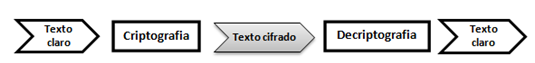
\includegraphics[width=0.8\textwidth]{processocriptografia.png}
\caption{Relação entre os termos  básicos de criptografia adaptado de~\cite{Schneier1995}.}
\label{fig:processocriptografia}
\end{figure}

Para realizar o processo de criptografia é necessário a utilização de um sistema criptográfico que é formado pelo conjunto de textos em claro, textos cifrados e chaves. Atualmente existem dois tipos de sistemas criptográficos: o de chave simétrica e o de chave assimétrica.

\subsection{Criptografia de Chave Simétrica}

A criptografia de Chave Simétrica pode ser definida como sendo aquela que utiliza uma chave única tanto para cifrar quanto para decifrar um texto claro~\cite{stallings2008}. Esse sistema de criptografia possui basicamente cinco elementos: Texto claro, que é a mensagem original; Algoritmo de criptografia, que o responsável por realizar as transformações no texto claro; A chave secreta, que é a chave compartilhada entre o emissor da mensagem e o receptor,utilizada como entrada para o algoritmo de criptografia; Texto cifrado, que é a mensagem em que foi aplicada o algoritmo criptográfico, é a saída e algoritmo de criptografia: Que é basicamente o mesmo algoritmo de criptografia só que executado de forma inversa. Para isso, ele aplica ao texto cifrado a chave secreta compartilhada, utilizada no momento da cifragem, e obtém o texto claro original. O processo do Sistema Criptografia de Chave Simétrica é ilustrado na figura~\ref{fig:criptografiasimetrica}

\begin{figure}[!htb]
\centering
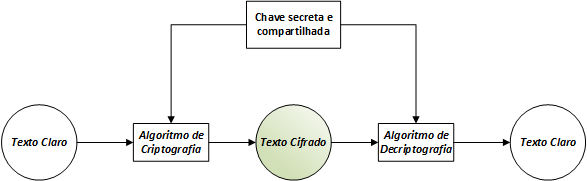
\includegraphics[width=0.9\textwidth]{criptosimetrico.png}
\caption{Processo de criptografia simétrica adaptado de ~\cite{stallings2008}.}
\label{fig:criptografiasimetrica}
\end{figure}

Existem dois tipos de algoritmos de criptografia de chave simétrica: os de cifras de fluxo e cifras de blocos. Cifras de fluxo, cifram e decifram dados bit a bit, ou seja, um bit a cada unidade de tempo, não sendo muito adequado a implementações em software. Já a cifras de blocos, realizam as mesmas operações em blocos de bits, sendo mais fáceis de implementar em softwares~\cite{Schneier1995}. São exemplos de algoritmos de criptografia de chave simétrica: AES(Advanced Encryption Standard), BlowFish, Triple-DES e DES (Data Encryption Standard).

\subsection{Criptografia de Chave Assimétrica}

A criptografia de Chave Assimétrica ou de chave pública é aquela que utiliza uma chave para criptografia e outra chave diferente, porém relacionadas matematicamente, para decriptografia~\cite{stallings2008}. Dessa forma, cada usuário possui um par de chaves, uma pública e outra privada, que são utilizadas no processo de ciframento e deciframento das mensagens. Na utilização dessa técnica, todos os participantes têm acesso a chave pública porém as chaves privadas devem ser de conhecimento apenas do seu proprietário, devendo permanecer protegida e secreta ~\cite{stallings2008}. A figura~\ref{fig:criptografiaassimetrica} exemplifica o processo de Criptografia de Chave Assimétrica.

\begin{figure}[!htb]
\centering
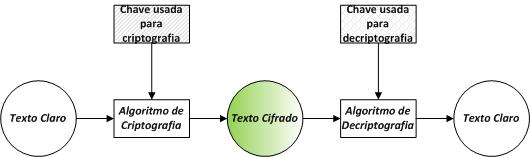
\includegraphics[width=0.9\textwidth]{criptografiaassimetrica.png}
\caption{Processo de criptografia assimétrica.}
\label{fig:criptografiaassimetrica}
\end{figure}

A criptografia assimétrica ou de chave pública pode ser utilizada tanto para prover a confidencialidade como para possibilitar a autenticidade da mensagem. Quando usada para prover a confidencialidade dos dados, a mensagem é criptografada com a chave pública do receptor e só pode ser decifrada com a chave privada do destinatário. Vários algoritmos de criptografia de chave pública foram propostos, porém os que mais se destacaram  tanto para  criptografia quanto para assinaturas digitais foram o RSA, ElGamal e Rabin~\cite{Schneier1995}.

\subsection{Funções de Hash}
Uma função de \emph{hash} é aquela que ao ser aplicada a uma mensagem de comprimento variável, produz como saída um valor \emph{hash}, de tamanho fixo~\cite{Schneier1995},também chamado de resumo de mensagem. Ela é amplamente utilizadas em aplicações criptográficas, tais como: assinaturas digitais, esquemas de proteção de senha e autenticação de mensagens. A finalidade da função de \emph{hash} é produzir um identificador único em um arquivo, mensagem ou bloco de dados. Para isso, ela deve satisfazer aos seguintes requisitos~\cite{stallings2008}:
\begin{itemize}
\item H pode ser aplicado a um bloco de dados de qualquer tamanho.
\item H produz uma saída de comprimento fixo.
\item Dado uma mensagem qualquer de entrada, deve ser fácil calcular o seu valor hash.
\item Para qualquer valor \emph{hash}(h) dado, é computacionalmente inviável encontrar x tal que H(x)= h. Ou seja,  deve ser resistente a primeira inversão, de forma que seja fácil gerar um código dada uma mensagem, mas muito difícil gerar um mensagem dado um código.
\item Para qualquer bloco dado x, é computacionalmente inviável encontrar y diferente x tal que H(y)= H(x). Isso é conhecido como resistência fraca a colisões.

\item É computacionalmente inviável encontrar qualquer par(x,y) tal que H(x)= H(y). Ou seja, deve possuir resistência forte a colisões.

\end{itemize}

Vários algorimos de \emph{hash} foram desenvolvidos ao logo dos anos. Como exemplo podem ser citados os algoritmos de resumo criptográfico ou MD(\emph{Message Digest}), desenvolvidos por Ron Rivest, e cuja a última versão foi o MD5. Porém a funções de \emph{hash} da familia MD foram considerados inseguros e devem ser evitados~\cite{forouzan2013redes}.

Outro exemplo, que merece destaque, são os algoritmos de hash seguro(SHA - \emph{Secure Hash Algorithm}). Eles foram desenvolvidos como alternativa a insegurança dos algoritmos MD(\emph{Message Digest}). O SHA é um padrão desenvolvido pelo Instituo Nacional de Padrões e Tecnologia (NIST-\emph{National Institute of Standards and Technology}). Atualmente, o SHA, encontra-se na versão 3,(SHA-3), sendo considerado o padrão recomendado para aplicações atuais e futuras~\cite{forouzan2013redes}.

\subsection{Assinatura digital}

A assinatura digital pode ser definida como o mecanismo de autenticação que permite que o criador de uma mensagem possa anexar um código que atue como assinatura e garanta origem e integridade da mensagem~\cite{stallings2008}. As assinaturas digitais podem ser geradas tanto por sistemas criptográficos assimétricos, usualmente os mais empregados, quanto simétricos. No caso da geração da assinatura digital com sistemas criptográficos assimétricos, o processo ocorre da seguinte maneira: a mensagem é criptografada com a chave privada do remetente, de forma que qualquer pessoa que possua a chave pública do remetente possa verificar a autenticidade da mensagem.

Porém a utilização da criptografia assimétrica e lenta, e como alternativa utiliza-se a combinação dos sistemas criptográficos com as funções de \emph{hash}. O que torna o processo mais rápido. Isso ocorre porque não se criptografa toda mensagem e sim apenas o resumo criptográfico, que é o resultado da aplicação da função de hash sobre a mensagem. Assinar um resumo criptográfico não é apenas mais eficiente do que assinar a própria mensagem, mas também uma defesa contra ataque do homem-do-meio, descritos na seção 3.5.4~\cite{goodrich2013introdução}.

Dessa forma, para gerar uma assinatura digital, utilizando a combinação da criptografia assimétrica com a função de \emph{hash}, deve-se seguir os seguintes passos, conforme descrito na figura~\ref{fig:esquemaassinaturadigital}. O emissor da mensagem aplica uma função de hash na mensagem que deseja enviar a um receptor, criando dessa forma, um resumo da mensagem com tamanho fixo.  Em seguida ele criptografa esse resumo com a sua chave privada e envia ao receptor juntamente com a mensagem original. O receptor, por sua vez, recebe o documento e realiza o processo de verificação da assinatura, de forma a determinar a autenticidade e integridade da mensagem enviada.  Para realizar essa verificação, ele aplica a mesma função de hash utilizada pelo emissor na mensagem original, e na sequência, ele utiliza a chave pública do emissor para decifrar o resumo de mensagem enviado, se o valor de \emph{hash} gerado pelo receptor  for igual ao valor de \emph{hash} enviado então ele terá a certeza que o documento não foi adulterado e que ele foi enviado realmente pelo emissor, detentor da chave privada. Em outras palavras a assinatura digital é válida.

\begin{figure}[!htb]
\centering
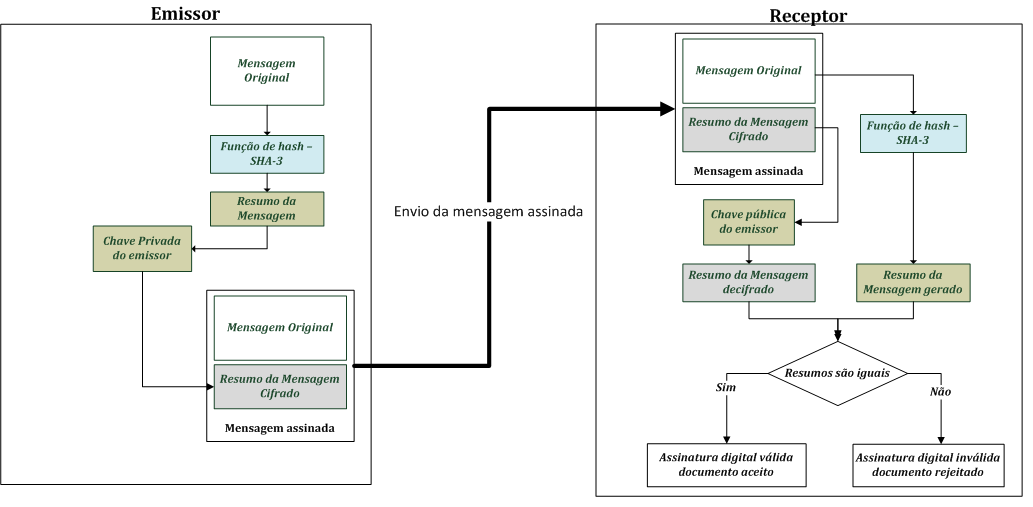
\includegraphics[width=0.9\textwidth]{esquema_assinatura_digital.png}
\caption{Processo de assinatura digital com função de hash.}
\label{fig:esquemaassinaturadigital}
\end{figure}

\subsection{Certificados Digitais}

Um certificado digital é um documento eletrônico que possui informações que comprovam a identidade do seu emissor. Esse documento eletrônico é gerado e assinado por uma terceira parte confiável, denominada Autoridade Certificadora (AC). Uma AC é responsável por associar uma chave pública a uma entidade(pessoa, processo, servidor etc)~\cite{forouzan2013redes}. Dessa forma, uma das finalidades de um certificado digital é garantir que a chave pública contida no certificado pertence à entidade à qual ele foi emitido, possibilitando assim, a identificação inequívoca das partes envolvidas em uma comunicação.

O padrão inicialmente adotado para os certificados digitais foi esquema X.509 que é uma recomendação do ITU-T(\emph{International Telecommunication Union}) e faz parte da série de recomendações X.500, que definem um serviço de diretório que mantém informações sobre usuários~\cite{stallings2008}.



\section{Vulnerabilidades em SOA}\label{sec:vulnerabilidadessoa}

Segundo~\cite{Verissimo2001}, hackers buscam por falhas e vulnerabilidades dos sistemas operacionais, aplicativos, software de rede e assim por diante. Usuários imprudentes ou administradores podem apresentar outras falhas, por causa da maneira como eles configuram ou executam os sistemas que operam. Esses problemas podem ocorrer em SOA. Para que se possa entender melhor esse contexto, são descritos a seguir conceitos que auxiliam o entendimento de vulnerabilidades.

Em relação a vulnerabilidades, pode-se afirmar que elas são falhas introduzidas, acidentalmente ou intencionalmente, durante o processo de desenvolvimento, configuração, operação e manutenção do sistema. Já ataques, são ações que exploram vulnerabilidades, podendo comprometer ou não as propriedades de segurança do sistema. E intrusão no sistema, é o resultado de um ataque bem sucedido no sistema.

%\begin{enumerate}[a )]
%	\item Vulnerabilidades são falhas introduzidas, acidentalmente ou  intencionalmente, durante o  processo de desenvolvimento, configuração, operação e manutenção do sistema;

%	\item Ataques são ações que exploram vulnerabilidades, podendo comprometer ou não as propriedades de segurança do sistema;

%	\item Intrusão no sistema é o resultado de um ataque bem sucedido.

%\end{enumerate}

A segurança aplicada a SOA é algo que deve ser continuamente buscado. Porém, essa tarefa é complexa e muitas vezes difícil. Isso decorre do fato de existirem muitas vulnerabilidades nos componentes de software. Com isso, para evitar que problemas de segurança ocorram, é necessário estar sempre revisando os métodos, técnicas e ferramentas que possibilitem verificar vulnerabilidades e propiciar segurança aos sistemas computacionais. A seguir serão descritos algumas vulnerabilidades que afetam a arquitetura orientada a serviços e que são citados no trabalho~\cite{JensenGHL2007}.

\subsection{Alteração das mensagens}

Neste tipo de ataque, as mensagens são interceptadas por um atacante que realiza alterações na mensagem toda ou em parte dela, afetando sua integridade. \emph{SQL Injection}, \emph{XML Injection} e \emph{XPath Injection} são exemplos de ataques que utilizam essa estratégia.

O \emph{SQL Injection}, é o ataque em que o atacante envia determinados parâmetros como argumentos das funções que, após processados pelo Web Service, originam  procedimentos SQL definidos pelo atacante~\cite{sonia2008}. Esses procedimentos podem retornar informações não previstas, alterar dados constantes nas bases de dados ou provocar indisponibilidade do próprio Web Service. Neste tipo de ataque podem ser executados comandos SQL inválidos.

No caso do \emph{XML Injection}, que é o ataque onde se procura modificar a estrutura XML de uma mensagem SOAP (ou qualquer outro documento XML), através da inserção de elementos XML~\cite{JensenGHL2007}. Isto pode ser usado para substituir os dados inseridos por usuário no mesmo documento. Nele, são aproveitadas as situações em que o processo de validação do XML não é efetuado corretamente, são inseridas tags num documento XML. As referidas tags XML podem alterar a estrutura do documento XML de tal forma que o comportamento da aplicação seja comprometido.

O \emph{XPath Injection}, é o ataque onde são inseridos parâmetros maliciosos no XPath, com o objetivo de realizar consultas a informações cujo acesso não foi autorizado. Segundo a W3C O XPath é uma linguagem utilizada para realizar consultas em documentos XML, e assim como SQL, também é suscetível a injeção de parâmetros~\cite{Sahba2007}.


\subsection{Negação de Serviços}

Ataques de negação de serviço são utilizados para impedir que o serviço funcione conforme o esperado, resultando em perda de disponibilidade~\cite{Siddavatam2008}. Esse ataque é focado em tornar indisponível (site, aplicativo de servidor, serviço). Se um serviço recebe um número muito grande de pedidos, ele pode parar de fornecer o serviço aos usuários legítimos.  Por exemplo, um ataque de negação de serviço pode ser realizado enviando uma grande quantidade de informações a um servidor com pedidos para consumir todos os recursos disponíveis no sistema, ou passando os dados de entrada mal formatados ao servidor de forma que ele pare de funcionar.

Ao contrário da maior parte dos ataques, esse não tem a intenção de invadir um computador para roubar informações confidenciais, seu objetivo é o de tornar inacessíveis os serviços providos pela vítima a usuários legítimos.

\subsection{Ataques de referências externas}

Neste tipo de ataque, o atacante consegue burlar as proteções criadas, como por exemplo, no caso de validadores de XML, e realiza a inclusão de referências externas que só serão consultadas após a validação do XML, mas antes da aplicação iniciar o seu processamento.

\subsection{Interceptação das mensagens}

Neste ataque, as mensagens são interceptadas e alteradas sem que qualquer das partes, emissor ou consumidor de serviço saiba que houve a interceptação. São exemplos deste ataque: \emph{Replay Attacks} e \emph{Man-in-the-middle}.

 No ataque \emph{Replay Attacks}, o atacante intercepta uma mensagem  e se faz passar pelo emissor. Dessa forma, ele pode reenviar mensagens que já tinham sido previamente enviadas, ou incluir partes de uma ou mais mensagens previamente enviadas numa nova mensagem (\emph{replay} de partes da mensagem). Já no caso do ataque \emph{Man-in-the-middle}, os dados trocados entre duas partes são de alguma forma interceptados, registrados e possivelmente alterados pelo atacante sem que as vitimas percebam as modificações.

\subsection{Descoberta de informação}

Neste tipo de ataque, as informações sobre os sistemas são descobertas e utilizadas para realizar um ataque, de acordo com o tipo de vulnerabilidade, que mais se adeque aos dados dos sistemas obtidos, tais como: tipo e versões do sistema operacional, localização de cópias de segurança, arquivos temporários, informações sobre os serviços dentre outras. Os principais ataques são:\emph{WSDL Scanning} e Ataques aos UDDI.

No ataque \emph{WSDL Scanning}, realiza-se uma varredura no documento WSDL, com a finalidade de se obter informações sobre os métodos, parâmetros e operações constantes no WSDL. Dessa forma, o atacante busca revelar informações sensíveis e possíveis falhas em um Web Service, o que lhe permite realizar um ataque bem sucedido~\cite{Moradian2006};

No caso do Ataques aos UDDI, o atacante analisa dados desprotegidos dos registros UDDI, e obtém detalhes relativos às funções disponibilizadas pelos Web Services e como acessá-los. Como, muitas vezes, os WSDL são gerados automaticamente por utilitários criados para exporem toda a informação disponível, relativa a um determinado método, é necessário ter alguma atenção na escolha/utilização desses utilitários de forma a ser possível proteger os Web Services desse tipo de ataque. Através da utilização de UDDI v.3.0.2 já é possível implementar alguma proteção relativa a este tipo de ataque. Essa versão já permite solicitar a identificação, autenticação e autorização das entidades antes de lhes dar acesso aos registos UDDI~\cite{sonia2008}.

\section{Protocolos de Autenticação e Autorização}
A comunidade web tem desenvolvido uma série de protocolos que abordam questões como identidade e confiança~\cite{Webber10}. Estes protocolos visam garantir que os sistemas possam interagir de forma segura. O principal benefício de se criar um serviço HTTP é a acessibilidade.  Uma vez que uma ampla gama de clientes em plataformas diferentes podem consumir os serviços HTTP~\cite{lakshmiraghavan2013pro}.

Para aplicar segurança em aplicações, geralmente e necessário fornecer mecanismos que permitam o cliente se identificar. Para isso, realiza-se o gerenciamento de identidade, que tem por finalidade permitir que os sistemas possam interoperar com segurança,divide-se basicamente em: Autenticação, que é o processo de descobrir a identidade de uma entidade por meio de um identificador e verificar a identidade através da validação de credenciais fornecidas pela entidade ~\cite{lakshmiraghavan2013pro}.E autorização que é o processo que analisa se um usuário após ser autenticado tem permissão para executar uma determinada ação.% O protocolo HTTP oferece dois tipos de autenticação, o  Basic e Digest.

%A autenticação Basic é um modelo baseado no desafio e resposta, sendo utilizada por servidores HTTP para validar a autenticação~\cite{franks1999}. Desta forma, quando o cliente tenta acessar algum recurso protegido, a sua identidade é requerida pelo servidor, o cliente então fornece a resposta codificada em base64 no header \emph{HTTP},  se a resposta for correta ela terá acesso ao sistema. Porém, por não criptografar o desafio, estando esse apenas codificado, faz com que ele seja vulnerável e sujeito a ataques, como por exemplo, os de repetição.

%Já na Digest, o processo é o mesmo que na autenticação básica. Sendo que seu mecanismo de autenticação é um pouco mais complexo, uma vez que ele gera um HASH, geralmente utilizando o algoritmo MD5, do desafio que será enviado pelo servidor ao cliente ~\cite{franks1999}. Apesar de ser mais seguro do que a autenticação básica, autenticação HTTP Digest também é vulnerável à ataques, como por exemplo o man-in-the-middle.  Para evitar esse problema, deve ser empregado a segurança na camada de transporte~\cite{Webber10}.

\subsection{OpenID}

O OpenID é um protocolo SSO(Single Sign-On)que permite a autenticação em diversos websites através de um Uniform Resource Identifier(URI). Ele foi desenvolvido em 2005 pela comunidade open source~\cite{Recordon2006}. Dentre as caracteríticas inerentes a ele podem ser destacadas:a descentralização e a identidade única, compartilhada com consumidores diferentes. Atualmente, encontra-se na versão 2.0.

OpenID é atraente por causa de sua simplicidade. Com apenas algumas interações, o cliente consegue solicitar e validar  uma autenticação um servidor OpenID e interagir com um serviço usando a alegação fundamentada. O fluxo do protocolo \emph{end-to-end} é apresentado na Figura~\ref{fig:openid}.

\begin{figure}[!htb]
\centering
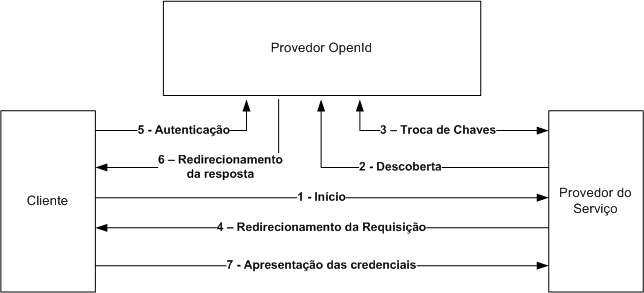
\includegraphics[width=0.8\textwidth]{openiddiagram.png}
\caption{Fluxo do protocolo OpenId, adaptado de~\cite{rfc6749}}
\label{fig:openid}
\end{figure}

\begin{enumerate}[1 )]
\item  Início, Um cliente envia um indentificador OpenID que alega possuir.

\item  Descoberta, o Provedor do Serviço descobre o provedor OpenID correspondente ao identificador OpenID apresentado pelo cliente.

\item Troca de chaves,  segredos são trocadas entre o Provedor do Serviço e o Provedor OpenID.

\item O Provedor do Serviço redireciona o cliente para provedor de OpenID, para que ele possa se autenticar.

\item Autenticação, o cliente se autentica no provedor OpenID. (A maneira em que a autenticação ocorre está fora do escopo OpenID.)

\item O Provedor de OpenID redireciona novamente o Cliente para o Provedor do Serviço.

\item Apresentação das credenciais, finalmente, a carga OpenID contendo a declaração de identidade validada é enviada para O Provedor do Serviço.

\end{enumerate}

\subsection{SAML}

O \emph{Security Assertion Markup Language - SAML} é uma especificação padrão para troca de credenciais,\emph{tokens} de segurança, que contém informações de autenticação e autorização, baseadas em \emph{XML}, que visam garantir a interoperabilidade entre diferentes sistemas. Foi desenvolvido em 2005 pela OASIS (OASIS,2005b; OASIS, 2005c). Ele está dividido no seguintes componentes: asserções, protocolos, ligações e perfis, que são descritos a seguir~\cite{Madsen2005}

Uma Asserção é um conjunto de informações que fornece uma ou mais informações feitas por uma autoridade \emph{SAML}. Ela é dividida em três tipos diferentes:  autenticação, atributo e decisão de autorização~\cite{Madsen2005,Nordbotten09,Bertino2010}. Uma asserção de autenticação, é aquela que afirma que determinada informação foi autenticada por um meio qualquer em determinado momento. Este tipo de asserção é geralmente emitido por uma autoridade \emph{SAML} denominada de fornecedor de entidades. A sua responsabilidade é a de autenticar consumidor do serviço e manter registros dos dados relacionados com a sua sessão, enquanto esta for válida. O atributo é a asserção que contém informações específicas de um determinado cliente. E finalmente a decisão de autorização, que são as informação sobre a decisão de permitir, ou não, o acesso a um determinado recurso por parte do consumidor do serviço.

Os Protocolos, nesse contexto são uma série de mensagens protocolares do tipo pedido/resposta que permitem um provedor de serviços, dentre outras coisas, solicitar a uma autoridade \emph{SAML}, uma ou mais asserções, pedir a autenticação de um usuário a um provedor de identidades e obter a asserções correspondentes.

As ligações, que são aquelas que realizam o mapeamento entre mensagens protocolares e as normas de comunicação entre sistemas, em linhas gerais, define como mensagens \emph{SAML} serão transportadas em cima dos protocolos padrão de mensagens e transporte.

Os perfis, são aqueles que definem um conjunto de restrições e ou extensões para o suporte da utilização de \emph{SAML}  em uma determinada aplicação.

Na versão 2.0 do \emph{SAML}, foram adicionadas uma série de novos recursos tais como os pseudónimos, gerenciadores de identidades e de sessões, metadados, encriptação, perfis de atributos, suporte a dispositivos móveis, mecanismos que permitem a aplicação de políticas de privacidade e métodos de pesquisa de provedores de identidades.

\subsection{OAuth}

O \emph{Open Authorization Protocol - OAuth} é um protocolo desenvolvido com o objetivo de solucionar os problemas relacionados com a gestão de identidades entre provedores de serviços. A primeira versão 1.0 foi lançada em 2007, e sua última revisão foi publicada em 2010, sendo especificada no Request For Comments (RFC)5849~\cite{oauth210}. Em 2012, a versão 2.0 do protocolo, \emph{OAuth 2.0}, foi lançada com objetivo de resolver problemas encontrados na versão 1.0, tais como escalabilidade e complexidade~\cite{rfc6749}.

Na última versão, 2.0, quatro papéis básicos são definidos e necessários para compreensão do fluxo de execução do protocolo, são eles: proprietário do recurso, que é a entidade que tem o poder de conceder a permissão de acesso, aos seus recursos, às outras entidades; O servidor de recursos, que é o responsável por hospedar e responder às solicitações de acesso a recursos protegidos, usando \emph{tokens} de acesso; Cliente, que é uma aplicação, que realiza solicitações de acesso de recursos protegidos, ao servidor de recursos, em nome do proprietário, dono do recurso, após a obtenção de sua autorização; E o servidor de autorização, que é responsável por emitir \emph{tokens} de acesso aos clientes, após autenticar e obter autorização do proprietário de recursos~\cite{rfc6749}.

%Na última versão, 2.0, quatro papéis básicos são definidos: proprietário do recurso, servidor de recursos, cliente e servidor de autorização~\cite{rfc6749}.

%O proprietário do recurso é a entidade que tem o poder de conceder a permissão de acesso, aos seus recursos, às outras entidades.

%O servidor de recursos é aquele responsável por hospedar os recursos protegidos, e tem a capacidade de responder às solicitações de acesso a recursos protegidos, usando \emph{tokens} de acesso.

%Já o cliente, é uma aplicação que realiza solicitações de acesso de recursos protegidos, ao servidor de recursos, em nome do proprietário dono do recurso após a obtenção da de sua  autorização.

%E por fim, o servidor de autorização, que é aquele que emite \emph{tokens} de acesso aos clientes, após autenticar e obter autorização do proprietário de recursos.

Na maioria dos casos, o papel do servidor de autorização e o servidor de recursos podem  ser representados por uma única entidade. A Figura~\ref{fig:diagramaoauth} apresenta de forma abstrata o fluxo do protocolo OAuth 2.0 e descreve a interação entre os quatro papéis.

\begin{figure}[!htb]
\centering
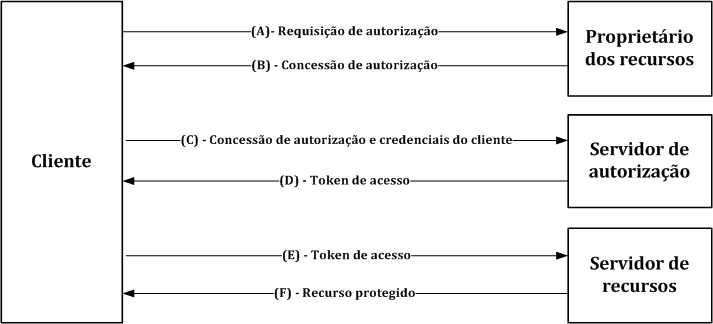
\includegraphics[width=0.8\textwidth]{diagrama_oauth2.png}
\caption{Fluxo do protocolo OAuth 2.0 adaptado de~\cite{rfc6749}}
\label{fig:diagramaoauth}
\end{figure}

\begin{enumerate}[a )]
        \item O cliente solicita a autorização do proprietário do recurso.
        \item O cliente recebe uma concessão de autorização, que representa a autorização fornecida pelo proprietário do recurso.
        \item O cliente solicita ao servidor de autorização um \emph{token} de acesso que pode ser usado para acessar os recursos protegidos. Durante este processo, o cliente fornece suas credenciais e a concessão de autorização para autenticar-se com o servidor de autorização.
        \item O servidor de autorização confirma a validade das credenciais do cliente e da concessão de autorização, se elas forem válidas, ele então fornece ao cliente um \emph{token} de acesso.
        \item O cliente solicita os recursos protegidos, hospedados no servidor de recursos, apresentando o \emph{token} de acesso.
        \item  O proprietário do recurso verifica a validade do \emph{token} de acesso e, se válido, ele atende ao pedido.

\end{enumerate}

\subsection{Traust}
\subsection{eXtensible Access Control Markup Language}
A eXtensible Access Control Markup Language (XACML) foi desenvolvida pelo OASIS Security Services Technical Commitee (SSTC). O padrão XACML define linguagens de marcação que permitem especificar políticas de segurança, requisições e respostas para decisões de controle de acesso, permitindo a organizações utilizarem essas políticas para controlar acesso a conteúdos e informações protegidas.

A linguagem para definição de políticas XACML é utilizada para descrever requisitos gerais de controle de acesso, e possui pontos de extensão para definição de novas funções, tipos de dados e combinações lógicas. As políticas de segurança XACML podem controlar o acesso a informação
utilizando identidade de clientes, o método de autenticação de clientes ou ainda uma porta pela qual um cliente se comunica.

O XACML difere de outras linguagens e padrões proprietários primeiramente pelo fato de ser um padrão aberto (Open-Standard). Segundo, por ser genérico, permite que possa ser usado para prover controle de acesso para sistemas completos bem como a um recurso específico. Finalmente, por
ser aplicável em conjunto com outros padrões, como o SAML, podendo formar a base para tomada de decisões.

O uso do XACML pode ser feito tanto em ambientes e aplicações proprietárias quanto públicas, podendo facilitar o processo de tomada de decisões e  proporcionar interoperabilidade entre diferentes plataformas e domínios.

\section{Síntese do capítulo}

Este capítulo apresentou conceitos básicos da arquitetura orientada a serviços. Foram abordados conceitos fundamentais da tecnologia Web Services, REST, sendo apresentadas as definições de sua estrutura. Além disso, foram descritos alguns protocolos de autenticação e autorização. No que tange a segurança em SOA, foram apresentados os conceitos básicos de segurança e elencadas algumas das principais vulnerabilidades que afetam a arquitetura orientada a serviços. No próximo capítulo, será descrito o protocolo de autenticação e autorização proposto e sua análise formal, utilizando para isso a lógica BAN.
